\documentclass[a4paper,10pt]{article}

\usepackage[headheight=0pt,headsep=0pt,footskip=3.5cm]{geometry}

\usepackage{epsfig}
\renewcommand{\figurename}{Figura}
\usepackage{float}

\usepackage{tocloft}
\renewcommand{\cftsecleader}{\cftdotfill{\cftdotsep}}
\renewcommand{\contentsname}{Contenidos}

\usepackage{amssymb}

\usepackage[hidelinks]{hyperref}

\usepackage{xcolor}

\begin{document}
\pagenumbering{gobble}
\tableofcontents

\pagebreak
\setcounter{page}{1}
\pagenumbering{arabic}
\section{Introducción}
En el presente informe se describen las tareas, realizadas en el laboratorio
GrIDComD, que fueron llevadas a cabo durante la ejecución de la Práctica Profesional
Supervisada correspondiente a la carreara Ingeniería en Computación por parte del autor de
este documento. El objetivo de la práctica fue diseñar e implementar un simulador de bajo costo
de las señales recibidas en vuelo por los satélites pertenecientes al sistema DCS.

\section{Lugar de trabajo}
\subsection{Descripción de la entidad}
\subsection{Organigrama}

\section{Sistema DCS}

La principal tecnología que el autor necesitó incorporar para la realización de la práctica, fue el conocimiento
sobre el Sistema Satelital Argentino de Recolección de Datos Ambientales (DCS). 
\par
Implementado por la comisión Nacional de Actividades Espaciales(CONAE), dicho sistema tiene como objetivo el
recolectar datos ambientales de distintos puntos del planeta, principalmente lugares inhóspitos y de difícil acceso. Este está formado
por tres segmentos:

\begin{itemize}
\item Segmento espacial: conformado por todos los elementos del sistema que se encuentran a bordo de satélites, este tiene como finalidad
recibir y almacenar los datos registrados, además de dar la posibilidad de obtenerlos desde la tierra, no sin antes preprocesarlos.
\item Plataformas: hace referencia a las plataformas que tienen como tarea recolectar datos de su entorno y transmitirlos a los satélites (DCP).
\item Segmento terrestre: compuesto por las facilidades que permiten descargar las lecturas almacenadas en los satélites y su disposición
a los usuarios para su análisis mediante servidores en línea o bien otros tipos de soportes de distribución de datos.
\end{itemize}
De este modo, los datos son leídos por las plataformas, quienes los transmiten a los satélites, donde son preprocesados para luego ser descargados 
y puesto a disposición de los usuarios mediante estaciones terrenas.


\subsection{Características de las señales}
Las señales transmitidas por las DCP poseen las siguientes características:
\begin{itemize}
\item Frecuencia de portadora de 401.55Mhz. Cabe destacar que si bien la posibilidad de colisión entre mensajes puede llevar a la pérdida de estos, 
los corrimientos de Doppler según la ubicación de cada DCP puede ayudar a separar estos en frecuencia.
\item Utiliza modulación PSK binaria con un $\theta$ de $\pm $ 1.1 rad $ \approx 63^o$.
\item Tasa de bits de 400bps.
\item Codificación Manchester.
\item Intervalo entre transmisiones de entre 30 y 220 segundos.
\end{itemize}

\subsection{Formato del mensaje}
El formato del mensaje enviado por las DCP se puede apreciar en la figura ~\ref{formatoMensaje}

\begin{figure}[H]
\centering
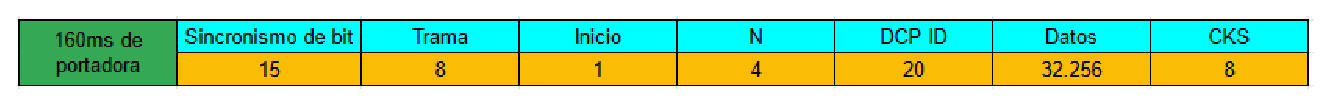
\epsfig{file=FigFormato.eps, width=14.0cm, height=1.1cm}
\caption{Formato del mensaje transmitido}
\label{formatoMensaje}
\end{figure}

Como se muestra, en primer lugar se transmite únicamente la señal portadora durante 160ms, con el fin de que el receptor detecte la señal y se sincronice con esta. Luego, se envía el mensaje en si, el cual consta de los siguientes campos:
\begin{itemize}
\item Sincronismo de bit: consta de 15 unos.
\item Trama: 8 bits que sirven para indicar al receptor que se está recibiendo un mensaje del sistema y solucionar la ambigüedad de $\pi$ en la fase.
\item Bit inicial: un uno que marcará el inicio de los bits a relevantes al mensaje a partir del primero luego de este.
\item N: campo de 4 bits que indica el tamaño en paquetes de 32 bits del campo de datos. Puede tomar valores entre 1 y 8, por esto el campo de datos puede tener entre 32 y 256 bits de largo.
\item DCP ID: 20 bits cuya función es identificar la plataforma que envía el mensaje.
\item Datos: los datos propiamente dichos.
\item CKS: checksum de 8 bits formada a partir de realizar el XOR entre todos los bytes que componen al resto de campos del mensaje. Este sirve para detectar errores en los bits recibidos.
\end{itemize}

\section{Implementación del simulador}
\subsection{Concepto}
Como fue mencionado, el objetivo de esta práctica fue el de implementar un simulador de bajo costo que imite las señales recibidas en vuelo por los satélites del sistema DCS, con el fin de utilizarse para probar receptores de estos. El principal motivo que impulsó esta tarea fue el hecho de que los simuladores disponibles en el mercado con las funcionalidades deseadas cuentan con costos prohibitivos.
\par
Este simulador está compuesto por una aplicación de escritorio (siendo esta  la principal tarea a realizar por el autor de este documento) capaz de generar las señales en banda base, las cuales son enviadas a través de la placa de audio de la computadora a un
generador de RF para ser moduladas en FM (dado que esta es la modulación que utiliza el sistema DCS), con una frecuencia de portadora igual a la mínima frecuencia observable por el receptor a probar. 

\begin{figure}[H]
\centering
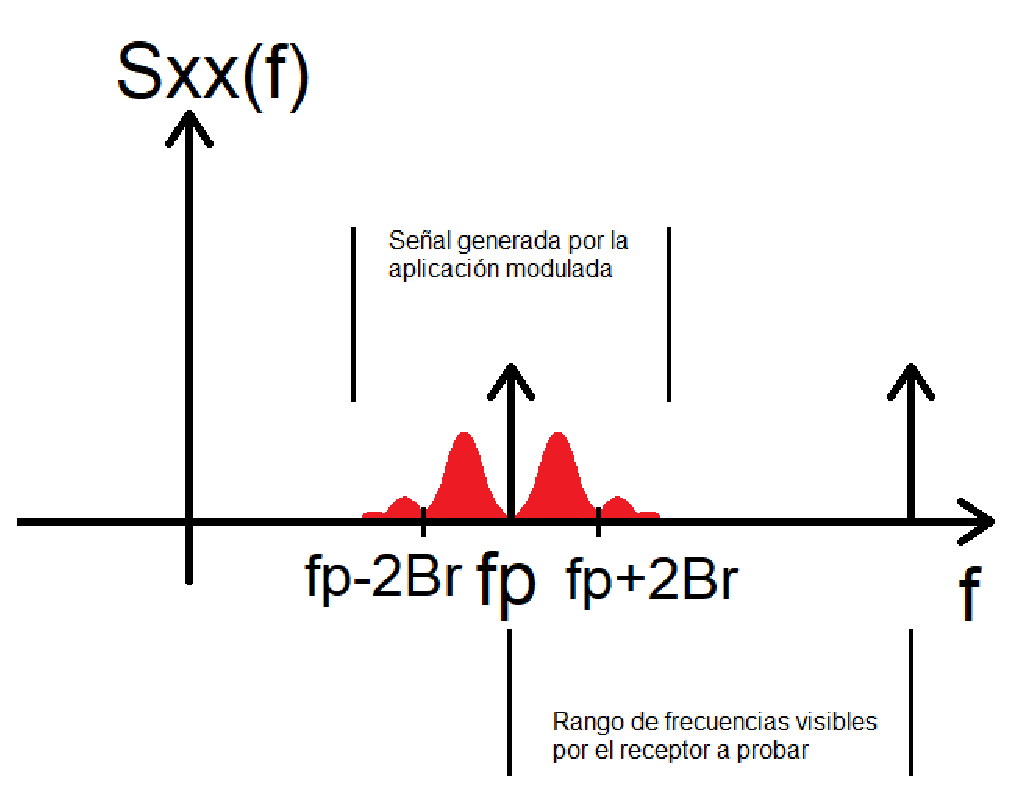
\epsfig{file=FigSim.eps, width=12.0cm, height=7.5cm}
\caption{Espectro de la simulación}
\label{espectroSim}
\end{figure}

\par
De esta forma, como se puede apreciar en la figura ~\ref{espectroSim}, el receptor "verá"  la parte derecha del espectro de la señal simulada modulada, permitiendo a la señal generada por la aplicación ser recibida por este. Cabe destacar que dado el hecho de que las frecuencias de muestreo de las placas de audio suele ser menor al rango de frecuencias de los receptores del sistema DCS (por ejemplo, una frecuencia de muestreo standar de estas placas es de 44,1Khz mientras que el receptor DCS del satélite SAC-C puede recibir en la banda de 401 a 403Mhz, osea, con un ancho de 2Mhz),  este simulador no permitirá probar este rango en su totalidad. Sin embargo, debería bastar para probar la capacidad de recepción de los receptores y su interacción con diferentes agentes que afectan a las señales que reciben.


\subsection{Software implementado}
Como fue mencionado, la principal tarea del autor dentro de el mencionado proyecto, fue la de implementar el software encargado de generar las señales en banda base. Cabe destacar que se tomó la desición de que las señales no sean generadas en tiempo real, sino
que el programa genere un archivo en formato wav con estas, de modo que se pueda reproducir varias veces una simulación de forma fácil, y no se generen problemas para la generación en tiempo real debido a recursos computacionales. Además, la frecuencia de muestreo
utilizada es de 44,1Khz, dado que esta se corresponde con una frecuencia estándar de las placas de audio, por donde se sacará esta señal.

\subsubsection{Tecnología}
La principal tecnología utilizada para este programa fue el lenguaje de programación Python. Esto se debe a que originalmente se iba a implementar con MATLAB u Octave, pero estos no brindaban herramientas satisfactorias para la interfaz de usuario. Por esto se optó por
Python, donde se puede trabajar con vectores de forma similar a dichos lenguajes con la ayuda de librerías, a la vez que se tienen numerosas opciones para hacer interfaces sofisticadas.
\par
Adicionalmente, se utilizaron las siguientes librerías de Python:
\begin{itemize}
\item NumPy: permite trabajar con vectores de forma similar a MATLAB u Octave.
\item SciPy: paquete de utilidades científicas varias, entre las que se encuentran las funciones Kron y Pwelch, además de la generación del archivo wav.
\item math: funciones matemáticas escenciales.
\item PySimpleGui: librería utilizada para realizar la interfaz de usuario.
\item random: generación de números aleatorios.
\item MatPlotLib: utilizada para generar gráficos, en este caso de de la DEP.
\end{itemize}

\subsubsection{Estructura de archivos}
El código fuente del programa  está formado por los siguientes archivos:
\begin{itemize}
\item main: programa principal, encargado de llevar las acciones correspondientes a los eventos de la interfaz.
\item UI: interfaz de usuario.
\item plat: clase utilizada para representar una plataforma.
\item enviroment: efectos ambientales.
\item signalGen: generación de mensajes, pulsos y señales.
\item simulador: motor de la simulación.
\end{itemize}
De desearse observar en detalle estos archivos, para así ver sus correspondientes funciones e implementación, esto se puede hacer visitando el siguiente  repositorio de Git Hub: 
\par
\textcolor{blue}{\url{https://github.com/tomyyn/PPS/tree/master/source}}

\subsubsection{Interfaz de usuario}
En la figura ~\ref{UI} se puede apreciar una captura de la interfaz de usuario del programa.

\begin{figure}[H]
\centering
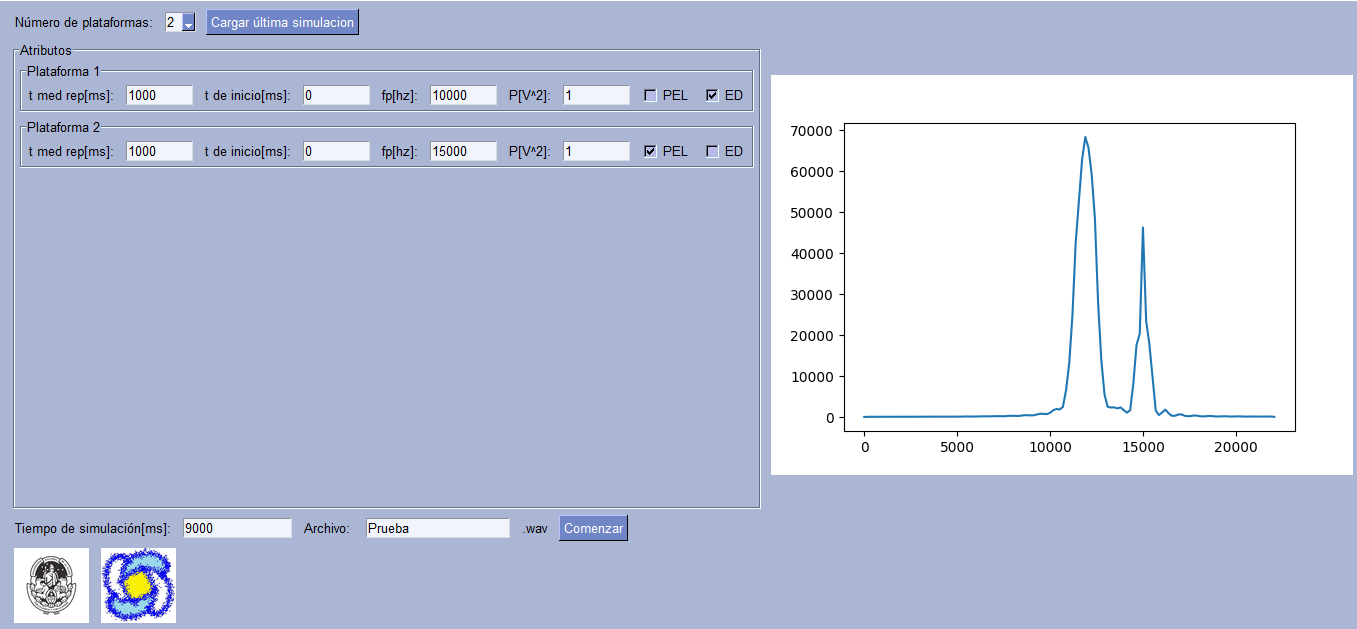
\epsfig{file=FigUI.eps, width=14.0cm, height=6.2cm}
\caption{Interfaz de usuario}
\label{UI}
\end{figure}

En la parte superior se pueden apreciar dos elementos principales: en primer lugar, un indicador del número de plataformas que se desean simular, en el cual se pueden indicar valores entre 1 y 8; En segundo lugar, un botón que permite cargar los parámetros de la última simulación realizada, lo que de no poder realizarse (potencialmente debido a no contarse con los datos de esta, almacenados en un archivo localizado en el directorio de la aplicación) se indica con un mensaje de error correspondiente.
\par
La parte central cuenta a su derecha con un panel para indicar los atributos de las plataformas a simular (mostrándose tantas como se indican en el correspondiente campo de la parte de arriba), estos son: tiempo medio de repetición en ms, tiempo de inicio en ms, frecuencia de portadora en hz, potencia en $V^2$ (cabe destacar que dado el hecho de que la simulación es normalizada, esto no representará su potencia real, sino que se usará principalmente para compararla con otras plataformas e indicar que tanto se verá afectada por la PEL) y si considera la pérdida en espacio libre y el efecto Doppler. A su derecha, esta parte presenta la DEP de una simulación luego de realizarla, esto permite apreciar principalmente que todo haya salido según lo indicado, y el corrimiento de Doppler.
\par
Finalmente, en la parte inferior se encuentran campos para indicar el tiempo total de simulación en ms, y el nombre del archivo donde se guardará esta. Adicionalmente se tiene el botón para comenzar la simulación, el cual de clickearse con parámetros vacíos o incorrectos (como puede ser una letra en el tiempo de simulación) indica que no se puede comenzar con un mensaje de error, el cual desaparece al comenzarse una simulación con parámetros completos y válidos.

\subsubsection{Funcionamiento}
El software comienza a generar las señales en banda base en el momento en que el usuario presiona el botón "Comenzar", siempre y cuando los parámetros ingresados sean válidos. Este funciona de la siguiente manera:
\par
En primer lugar, se crean los objetos y estructuras necesarias para esta simulación. Esto se refiere a, por un lado, instanciar las plataformas a simular (cada una con sus parámetros correspondientes);  Por otro, crear un vector capaz de alojar toda la simulación (inicializado con todos sus valores en 0), teniendo este un número de elementos basado en la duración de esta y la frecuencia de muestreo, sumando un segundo en caso de que una transmisión comience cerca del final.
\par
En segundo lugar, se obtienen las simulaciones de todas las transmisiónes de una plataforma (cada transmisión constando de generar un mensaje cuyo contenido está formado por un número aleatorio de "escaleras", convertirlo en pulsos, y estos en la señal, teniendo en cuenta los efectos ambientales de ser necesario). y se suman al vector de la simulación con el desplazamiento correspondiente. Esto es realizado para cada una de las plataformas.
\par
Finalmente, una vez el vector de la simulación se encuentra completo con todas las transmisiones de las distintas plataformas, este es normalizado y finalmente escrito en un archivo wav  para su reproducción.

\subsubsection{Implementación de efectos ambientales}
Resulta pertinente el comentar como fueron implementados los efectos ambientales considerados en el simulador, cuyas implementaciones fueron pensadas para ser simples desde un punto de vista computacional:
\begin{itemize}
\item Perdida en espacio libre: la pérdida en espacio libre en el sistema DCS puede alcanzar un valor máximo de 12dB. De este modo, para cada transmisión se obtiene un número al azar entre 1 y 3.98107170553 y se divide por este a todas sus muestras, lo que corresponde a una pérdida de entre 0dB y 12dB en potencia. Esta simple implementación se debe a que el cambio de degradación a lo largo de una transmisión no debería ser notorio debido a su corta duración.
\item Efecto Doppler: en este caso, cada plataforma cuenta con un perfil de Doppler (estando todos estos precargados en el programa) y un punto de comienzo para este (simbolizando en que punto de su recorrido se encuentra la plataforma con respecto al satélite al momento de comenzar la simulación). Con los elementos mencionados, para cada muestra de una determinada transmisión se agrega el valor de Doppler correspondiente a la frecuencia de portadora según el instante de tiempo y su perfil. Cabe destacar que una vez pasa el tiempo correspondiente a la duración del perfil de Doppler, este se repite de manera idéntica ya que el recorrido relativo de una plataforma y el satélite es periódico. La principal razón por la que en este caso se usa un valor de efecto Doppler para cada muestra de la transmisión en contraposición al uso de un solo valor por transmisión para la PEL, es probar que el receptor puede mantener el enganche con los cambios de frecuencia de portadora recibida,  sobre todo para el caso en el que haya un salto brusco dado a que una plataforma pase por el punto mas cercano al satélite durante una transmisión, causando que se pase del máximo valor negativo al máximo positivo del efecto Doppler, cosa que el receptor debería ser capaz de soportar.
\end{itemize}

\subsection{Pruebas}
Para las pruebas del sistema, las cuales tuvieron lugar en el laboratorio, se generó en primer lugar una simulación con una sola plataforma cuya frecuencia de portadora era de 20khz. 

\begin{figure}[H]
\centering
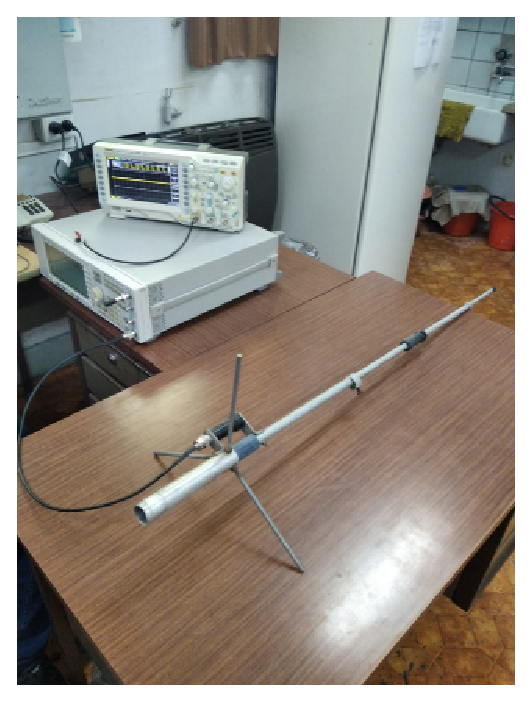
\epsfig{file=FigTest.eps, width=4.0cm, height=6.2cm}
\caption{Osciloscopio y generador de RF utilizados en las pruebas}
\label{Test}
\end{figure}

Esta simulación fue en primer lugar reproducida y sacada por un parlante para ser escuchada, lo que se realizó con éxito. Luego, se sacó esta señal por el jack de audio hacia el osciloscopio apreciable en la figura ~\ref{Test}, donde se verificó que las transmisiones tengan forma al comienzo de sinusoide debido a transmitir únicamente la portadora, y luego de señal modulada, lo que de nuevo tuvo éxito.
\par
Una vez corroborrado que la señal en banda base se podía escuchar y la forma de las transmisiones era correcta, se pasó a introducir la señal en el generador de RF visto en la figura ~\ref{Test} y modularla en AM, con el fin de apreciar la simulación en pasa banda desde una notebook con un dongle conectado y usando el software SDR\#. En primera instancia se trató de modular a 400Mhz, pero esto no dio buenos resultados dado que en frecuencias cercanas se encontraba un nivel apreciable de ruido. Debido a esto, se la movió la frecuencia de la modulación a  400,05Mhz, tal que las transmisiones de la simulación se encuentren centradas en 400,07Mhz. Esto último dio como resultado poder ver las transmisiones en el espectro, como se puede apreciar en \textcolor{blue}{\href {https://drive.google.com/file/d/1FieeQKkBJIfpKAu_4E4Ik1SV4s9q1Qw6/view?usp=sharing}{este}} video. Cabe destacar que también se pudo ver como la forma del espectro para las transmisiones era la deseada.
\par
Por último, se generó otra simulación donde se agregó una segunda plataforma centrada 10Khz que tuviera en cuenta el efecto Doppler. En  \textcolor{blue}{\href {https://drive.google.com/file/d/1FfI8xw6hzwwgcrzLQBHW1-g3nXa6ZuWW/view?usp=sharing}{este}} video se ve como se podían ver ambas. Adicionalmente, si bien en el video no se llega a notar, a lo largo de la simulación podía apreciarse como la segunda plataforma se iba desplazando en el espectro con cada simulación debido al efecto Doppler.


\section{Organización y experiencia}
\subsection{Orden de trabajo}
El orden de trabajo realizado puede separarse en tres etapas principales.
\par
La primera etapa fue la fase de estudio. En esta se estudió todo lo relacionado con el sistema DCS además de repasar conceptos relacionados de las comunicaciones digitales. Todo el material y fuentes necesarios fueron provistos por los directorres. Fue en
esta donde también se terminó de fijar la tecnología con la cual se terminó desarrollando el simulador, la cual requirió un estudio adicional para pulir conocimientos por parte del autor.
\par
La segunda etapa fue donde tomó lugar la implementación en sí. Durante este tiempo se fue implementando el simulador a la par de que se ultimaban detalles de este y se tenían revisiones periódicas con los directores para verificar el progreso y que se
estaba implementando lo correcto.
\par
La tercera etapa fue en la cual se realizaron las pruebas al simulador, las cuales fueron detalladas anteriormente.
\par
Cabe destacar que en cada etapa se asumieron las responsabilidades correspondientes a las tareas mencionadas, teniendo un mínimo de progreso a cumplir entre cada reunión.
\subsection{Organización de reuniones y comunicación}
Respecto a la organización de reuniones con los directores, estas tuvieron un espaciamiento de entre una y tres semas según las posibilidades de reunirse y los avances realizados. Estas reuniones fueron tanto virtuales como presenciales, teniendo como lugar el mismo laboratorio, según la situación de contagios en cada momento.
\par
Mas allá de lo mencionado, también tuvo lugar la comunicación a través de e-mail tanto para coordinar las actividades como para resolver dudas menores sin tener que esperar a las reuniones.
\par
Además, los directores contaban con acceso al repositorio de GIT con el proyecto y sus tareas relacionadas, por lo que podían observar el progreso a través del versionado.
\subsection{Experiencia con el personal}
En cuanto al personal del laboratorio, este se mostró abierto y dispuesto a ayudar desde el primer momento. Debido a esto, la integración resultó sencilla sin ninguna complicación de por medio. Adicionalmente, el equipo presentaba una gran flexibilidad en cuanto a tiempos,
lo que facilitó notablemente la cuestión de llevar a cabo la práctica a la par de los estudios, sobre todo en los momentos de mayor demanda por parte de lo segundo.

\section{Conclusiones}
Esta experiencia resultó altamente enriquecedora desde un punto de vista tanto personal como profesional, al presentar un ambiente nuevo, con relaciones nuevas y brindar una interacción mas cercana con el mundo de las comunicaciones digitales. 
Si bien en un principio el trabajo resultaba un poco intimidante, el ameno ambiente del laboratorio ayudó a rapidamente apaciguar ese temor gracias a la buena disposición de sus integrantes. En cuanto a los conocimientos adquiridos, estos no solo fueron técnicos, sino que 
también se incorporaron saberes relacionados al ambiente profesional, a las relaciones en el trabajo y valores. 
\par
Una de las principales enseñanzas no técnicas es que si bien no está mal utilizar cosas ya implementadas, y es incluso necesario, no hay que menospreciar lo que
puede hacer uno mismo y la importancia de tener el implementar algo como una opción, sobre todo cuando las opciones disponibles no resultan adecuadas.
\par
En cuanto a su significado, esto fue una oportunidad para poner a prueba varios conocimientos adquiridos durante la carrera, y  durante el proyecto, ya que también demostró que uno siempre tiene cosas por aprender. Adicionalmente, funcionó como un primer 
acercamiento a un ambiente real de trabajo, en el cual se tenían responsabilidades cuyas consecuencias iban mas allá de la nota en una materia. 
\par
Además, fue una oportunidad para desarrollar algo para lo que si bien se tenían claros los objetivos, inicialmente no se contaba con
muchas cosas resueltas, tanto en cuanto a tecnologías como a implementación, por lo que tener a cargo el resolver varios aspectos fue un gran aprendizaje también. Es importante remarcar también que la única experiencia laboral previa que se tenía era en el rubro de la docencia, por lo que fue la primera vez trabajando en una organización con estas características.
\par
En conclusión, considero que esta práctica me aportó muchísimas cosas que me acompañarán en el resto de mi vida profesional y me ayudarán a desenvolverme en mi carrera, sin duda una experiencia muy gratificante como la última antes de recibirme como ingeniero, y que 
considero que mas que un final, es un comienzo.
\end{document}